\section{System Architecture}
\label{sec:system-architecture}

\subsection{Architecture style}
\status{IMPLEMENTED}

The system is a classical \textbf{three-tier client--server architecture}:

\begin{enumerate}
    \item \textbf{Presentation tier} -- React single-page application, rendered client-side, communicating exclusively over JSON REST.
    \item \textbf{Application tier} -- Spring Boot stateless REST API implementing authentication, authorisation and business rules.
    \item \textbf{Data tier} -- MySQL relational store accessed through JPA/Hibernate.
\end{enumerate}

\noindent There is no message broker, cache server, search engine, file store or background job runner in the repository: every interaction is a synchronous HTTP request/response cycle.

\begin{figure}[H]
    \centering
    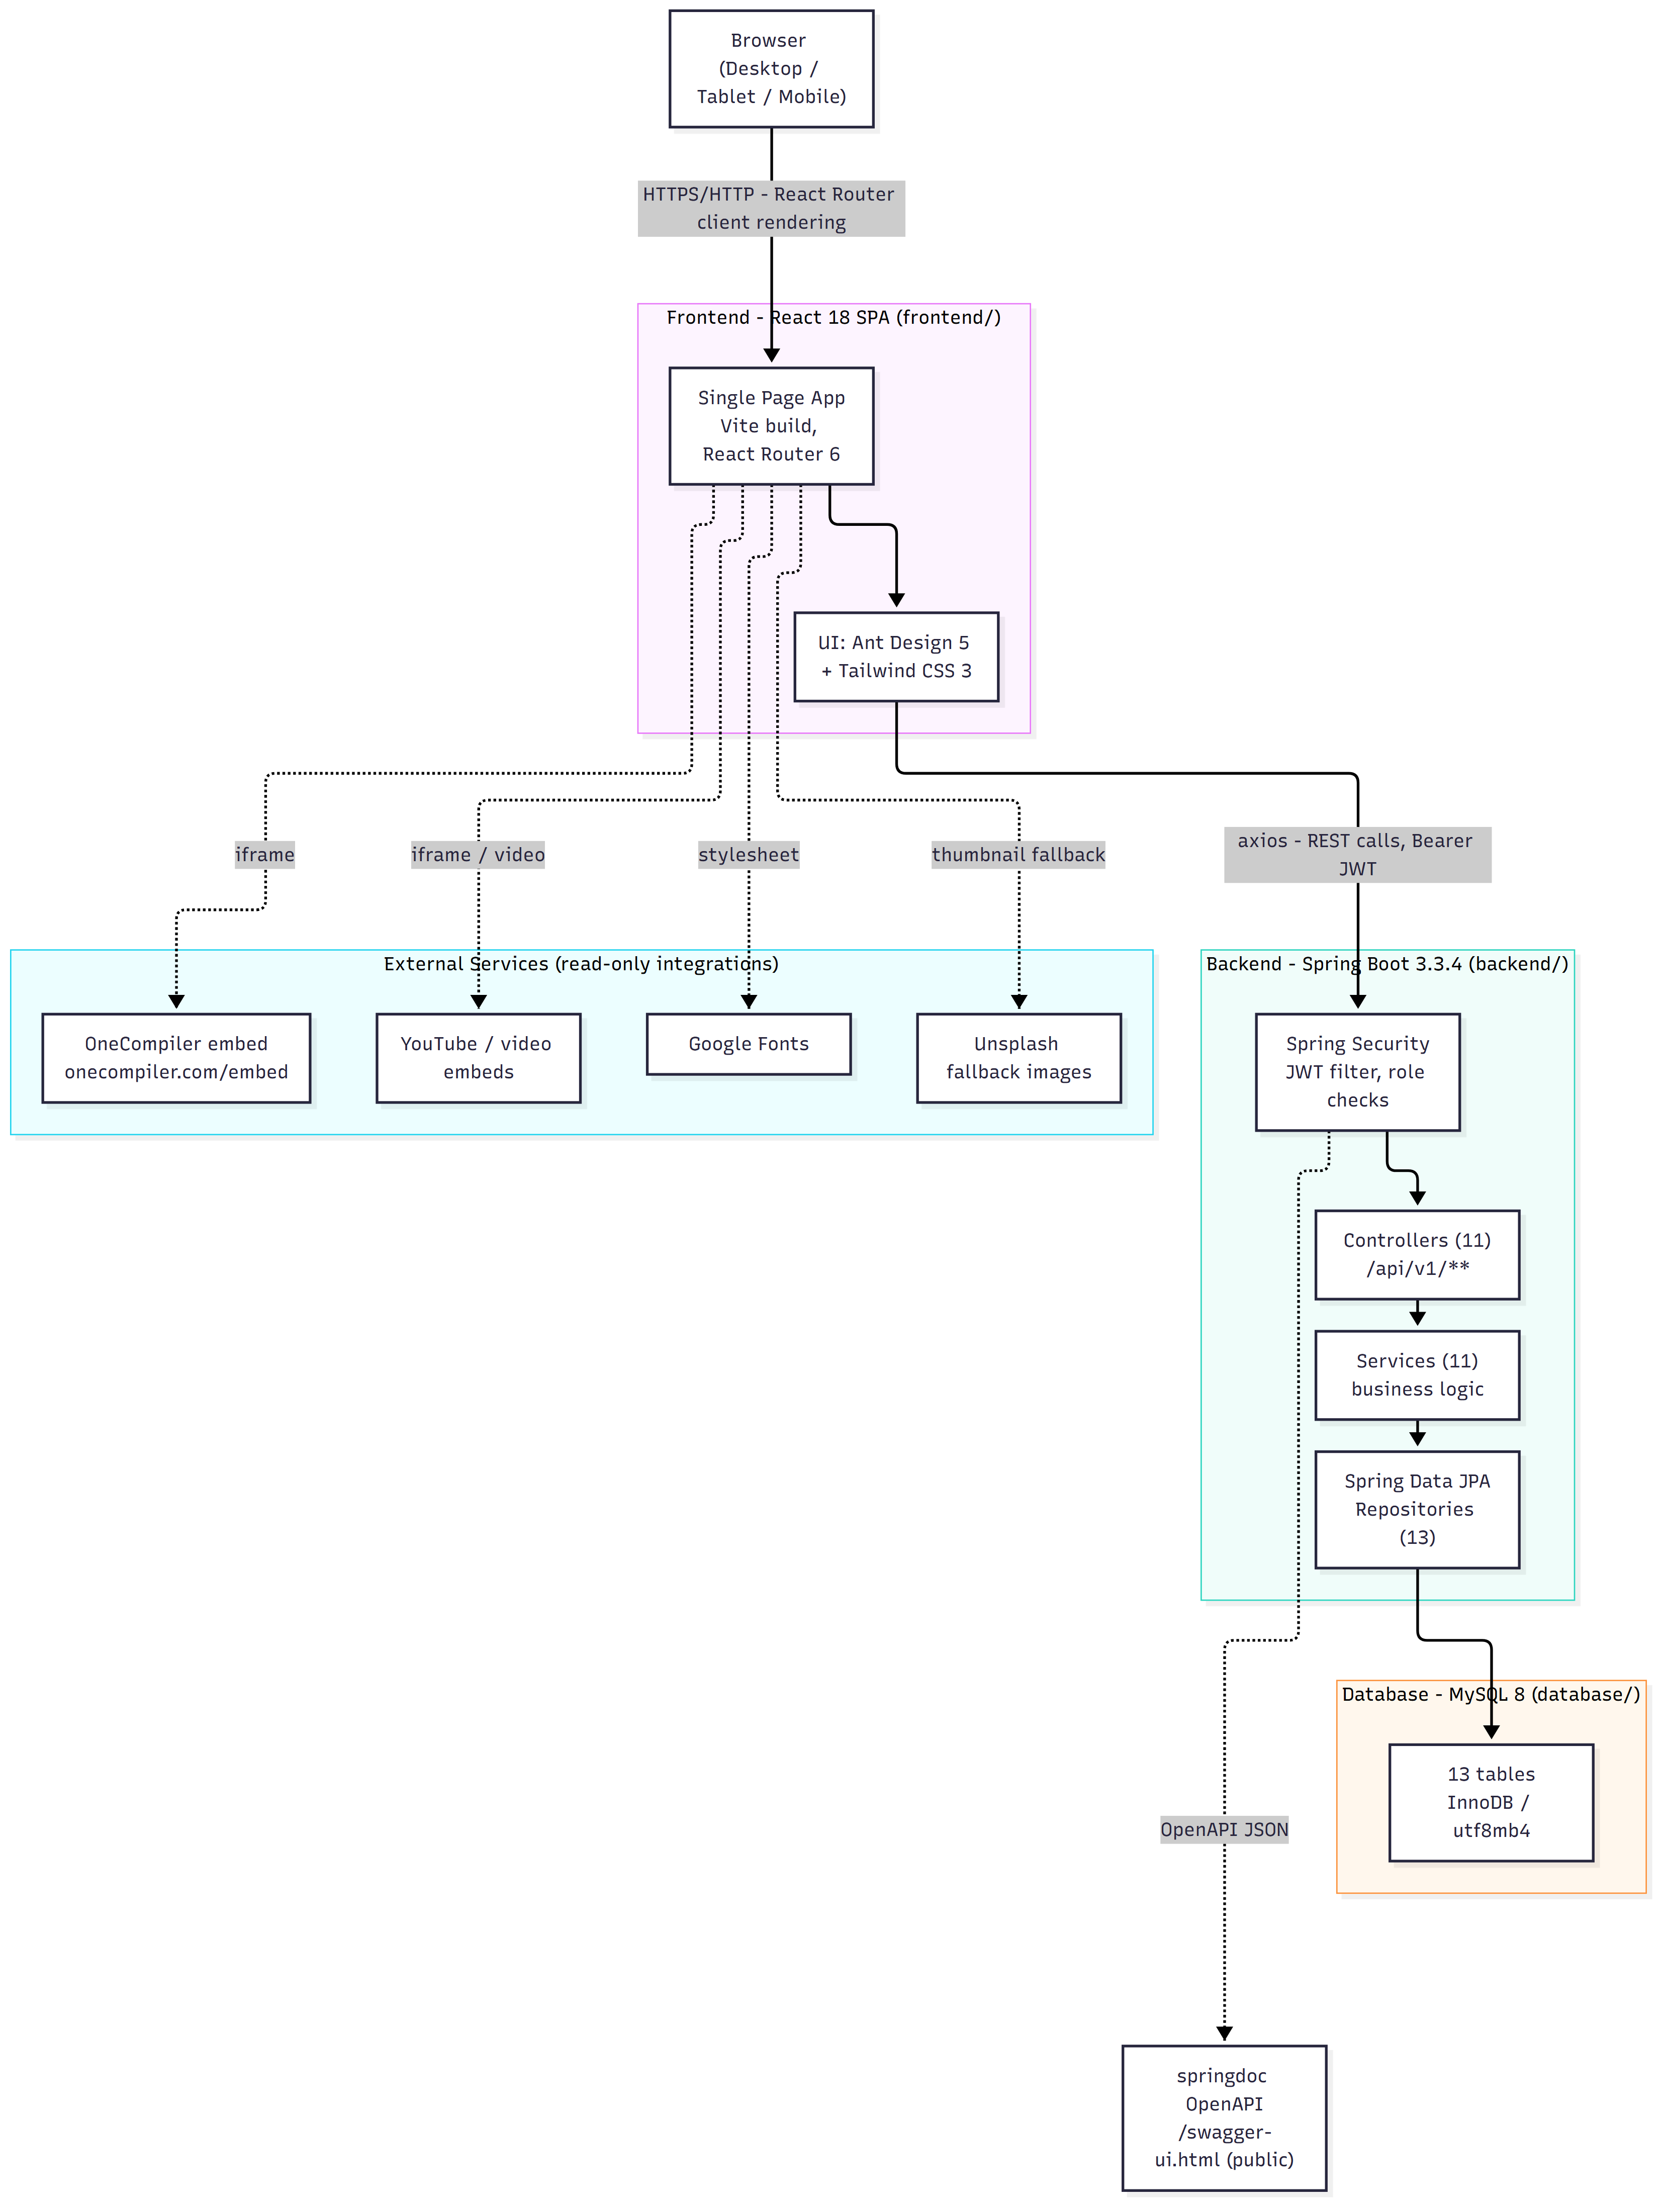
\includegraphics[width=0.9\textwidth]{diagrams/system-architecture.png}
    \caption{System architecture -- runtime components and external dependencies}
    \label{fig:sysarch-full}
\end{figure}

\subsection{Runtime components}
\begin{table}[H]
\centering
\caption{Runtime components and responsibilities}
\label{tab:runtime-components}
\begin{tabular}{@{}L{3.6cm}L{5.4cm}L{5.2cm}@{}}
\toprule
\textbf{Component} & \textbf{Responsibility} & \textbf{Key evidence} \\
\midrule
Browser & Renders SPA, holds session in \code{localStorage} & \pathref{frontend/src/context/AuthContext.jsx} \\
Vite dev server (dev) & Serves module graph on :3000, proxies \code{/api} & \pathref{frontend/vite.config.js} \\
Static host (prod) & Serves built \code{dist/} bundle & \code{npm run build} script \\
Axios client & Adds Bearer token, unwraps envelopes, maps errors & \pathref{frontend/src/api/client.js} \\
Spring Security filter chain & JWT validation, role enforcement, CORS & \pathref{backend/src/main/java/com/example/lms/config/SecurityConfig.java} \\
REST controllers (11) & HTTP binding + validation & \pathref{backend/src/main/java/com/example/lms/controller/} \\
Services (11) & Business rules, transactions & \pathref{backend/src/main/java/com/example/lms/service/} \\
JPA repositories (13) & Persistence & \pathref{backend/src/main/java/com/example/lms/repository/} \\
MySQL & Durable storage, constraints, indexes & \pathref{database/schema.sql} \\
springdoc & OpenAPI JSON + Swagger UI & \pathref{backend/src/main/java/com/example/lms/config/OpenApiConfig.java} \\
\bottomrule
\end{tabular}
\end{table}

\subsection{Trust boundaries}
\status{IMPLEMENTED (design) / PARTIAL (enforcement)}

\begin{enumerate}
    \item \textbf{Browser $\leftrightarrow$ API:} the only trusted client boundary. Tokens are issued and validated here; everything crossing this boundary is untrusted input validated by Bean Validation.
    \item \textbf{API $\leftrightarrow$ Database:} credentials via environment (\code{DB_URL} etc.); application connects as configured datasource user.
    \item \textbf{Client-side state:} \code{localStorage} tokens are convenience state, not a security boundary -- contract section 13 explicitly states frontend guards are not security controls.
    \item \textbf{Third-party origins:} OneCompiler iframe, YouTube, Google Fonts, Unsplash are outside the trust boundary and receive no user secrets.
\end{enumerate}

\subsection{Deployment view}
\status{PARTIAL}

The only artefact is \pathref{backend/Dockerfile} (multi-stage: JDK 21 alpine build with Maven, then JRE 21 alpine runtime, \code{EXPOSE 8080}). The frontend has no Dockerfile; no compose file ties components together; no production topology is defined. The verified development topology is: MySQL on \code{localhost:3306} + \code{./mvnw spring-boot:run} on :8080 + Vite on :3000. See Section~\ref{sec:deployment}.

\subsection{Architecture decisions (observed)}
\status{INFERRED (decisions are implicit in code)}

\begin{itemize}
    \item \textbf{Stateless JWT over server sessions} -- enables stateless scaling but forfeits revocation (see Section~\ref{sec:authentication}).
    \item \textbf{Monolith over microservices} -- one deployable JAR; appropriate for current scale; contract forbids unagreed technology changes.
    \item \textbf{Server-authoritative scoring} -- correctness and certificates decided in the backend; client is display-only.
    \item \textbf{Hibernate \code{ddl-auto: update}} over versioned migrations -- fast iteration, but schema history is not tracked (risk recorded in Section~\ref{sec:technical-debt}).
    \item \textbf{Static practice dataset} -- practice features shipped without backend work by explicit, documented design.
\end{itemize}
